%______________________________________________________________________________________________________________________
% @brief    LaTeX2e Resume for Kamil K Wojcicki
\documentclass[margin,line]{resume}
\usepackage[latin1]{inputenc}
\usepackage{graphics}
\usepackage{amsmath,amssymb}
\usepackage{gensymb}
\usepackage{amsthm}
\usepackage{wrapfig,lipsum,booktabs}
\usepackage{caption}
\usepackage{subcaption}
\usepackage{tabulary}
\usepackage{epigraph}
\usepackage{mwe}
\usepackage[autostyle]{csquotes} 
\usepackage{lipsum,lmodern}
\usepackage[skins]{tcolorbox}
\usepackage{pgf,tikz}
\usetikzlibrary{arrows,shapes,backgrounds,fit}
\usetikzlibrary{arrows,automata}

\usepackage{fancyvrb}
\usepackage{listings}
\usepackage{color}
\usepackage{eurosym}
%______________________________________________________________________________________________________________________
\begin{document}
\name{\Large Simon Holmbacka. PhD -- Resume\flushright{13 July 2016}}
\begin{resume}
\begin{picture}(320,0)
\put(350,-130){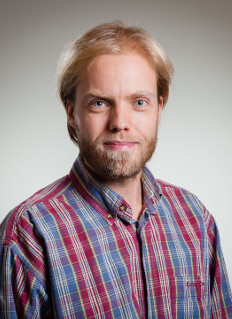
\includegraphics[scale=0.8]{simon.jpg}}
\end{picture}
    %__________________________________________________________________________________________________________________
    % Contact Information
    \section{\mysidestyle Contact\\Information}

    Embedded Systems Laboratory                         	     \vspace{0mm}\\\vspace{0mm}%
    Faculty of Science and Engineering                           \vspace{0mm}\\\vspace{0mm}%
    \AA{}bo Akademi University, Finland			       		\vspace{0mm}\\\vspace{-4.5mm}%
    
\small{
    Frantsinkatu 2 B 9			\vspace{0mm}\\\vspace{0mm}%
    20540 Turku, Finland		\vspace{0mm}\\\vspace{0mm}%
    Tel: +358 50 5310467		\vspace{0mm}\\\vspace{0mm}%
    Email: sholmbac@abo.fi		\vspace{0mm}\\\vspace{0mm}%
    Gender: male			\vspace{0mm}\\\vspace{0mm}%
    Time of birth: 24.01.1986		\vspace{0mm}\\\vspace{0mm}%
    Place of birth: Jakobstad, Finland	\vspace{0mm}\\\vspace{0mm}%
    Nationality: Finnish		\vspace{0mm}\\\vspace{-4.5mm}%
    }

\section{\mysidestyle Position}
    \textbf{Post-Doc Researcher}	\hfill \textbf{January 2016 -- }\vspace{0mm}\\\vspace{0mm}%
    \AA{}bo Akademi University Finland. Faculty of Science and Engineering,\\ Embedded Systems Laboratory.\\
    Task: \textit{Post-doc research and teaching}\\
    \textbf{Wissenschaftlicher Mitarbeiter} \hfill \textbf{September 2015 -- }\vspace{0mm}\\\vspace{0mm}%
    Fernuniversit\"{a}t in Hagen, Germany. Lehrgebiet Parallelit\"{a}t \& VLSI\\
    Task: \textit{Post-doc research and teaching}

\section{\mysidestyle Education}

    \textbf{\AA{}bo Akademi University}, Finland \vspace{2mm}\\\vspace{1mm}%
    \textsl{Doctor of Technology in Computer Engineering (26 Jan. 2016, Turku, Finland)} \hfill \textbf{ 2011 -- 2015}\vspace{-3mm}\\\vspace{-1mm}%
    \begin{list2}
        \item Faculty: Science and Engineering
	\item Major: Embedded Computer Systems
	\item Minor: Software Engineering
	\item Minor: University Pedagogics
	\item Thesis: \textit{Energy-Aware Software for Many-Core Systems} \textbf{Grade:} Honorary Grade
	\item Reference: Prof. Johan Lilius \textit{johan.lilius@abo.fi}
    \end{list2}\vspace{-1.5mm}
    \textsl{Master of Science in Computer Engineering (31 Mar. 2011, Turku, Finland)} \hfill \textbf{ 2009 -- 2011}\vspace{-3mm}\\\vspace{-1mm}%
    \begin{list2}
        \item Institution: Information Technologies
	\item Major: Embedded Computer Systems
	\item Minor: Control Engineering
	\item Minor: Software Engineering
	\item Thesis: \textit{Task Migration in Virtualized Multi-Core Real-Time Systems} \textbf{Grade:} 5/5
    \end{list2}\vspace{-1.5mm}
    \textsl{Bachelor of Science in Computer Engineering (6 Oct. 2009, Turku, Finland)} \hfill \textbf{ 2006 -- 2009}\vspace{-3mm}\\\vspace{-1mm}%
    \begin{list2}
        \item Institution: Information Technologies
	\item Major: Embedded Computer Systems
	\item Minor: Software Engineering
    \end{list2}\vspace{-1.5mm}

% \section{\mysidestyle Research\\Interests}
% Energy-Aware Software, Power Management, Parallel Programming, Many-Core Systems, Control Theory    
%    
%     
\section{\mysidestyle About me}
I come from the small city of Jakobstad in the mid west of Finland from which I moved to Turku to study computer engineering in 2006.
I completed my Master's degree in 5 years (2006 -- 2011) and my PhD in 4 years (2011 -- 2015) from \AA{}bo Akademi University in Turku, Finland.

\hspace{-2.0cm} \textit{Technical}\\
I have worked extensively in the areas of embedded systems, runtime systems, power management and many-core platforms, which includes foremost low level system programming (usually in C). 
Furthermore I have experience in object oriented programming languages, mostly C++ and Java, and I have of course stumbled upon some Python, C\#, .net, VB, Java script, xml and assembly progamming.
I have worked with system modeling, mathematical optimization and control theory including NLP optimization, digital filtering, plane fitting methods, control theory and its underlying mathematics. 
This means that I have very good knowledge of Matlab, its toolboxes and system simulation in Simulink.
On the hardware side, I have excellent knowledge of ARM and Intel platforms in particular, and system/kernel programming using Linux. 
I have been hacking with the Linux kernel since I was 16 years old and know this world in and out.
From my PhD work, I created an Android app called ``Low Energy Player'' freely available on Google Play.
On further lower level I have worked with real-time operating systems like FreeRTOS during my PhD and I have also build many hobby projects from scratch using micro controllers such as an audio synthesizer complete with a midi interface and USB driver running on an 8-bit AVR.
\clearpage

\hspace{-2.0cm} \textit{Project Work}\\
In the 4 years of making my PhD I have published over 15 international peer reviewed scientific articles, one of which I received the best paper award for in 2014. 
I worked in the European FP-7 project RECOMP from 2011 -- 2014 and in the national Tekes project ParallaX from 2014 -- 2016, in which I worked together with universities and
international IT companies like Wittenstein ltd., UK and Seven Solutions, Spain on programming and integration tasks.
I am a very good team worker, which has shown in co-operations with 7 different universities in 4 countries during this time for my thesis, and outside of my thesis I have published work together with 12 different institutions and co-authored work together with over 30 people.
I have visited more than 30 countries in my thesis work, and I find it very easy to join a team and start working on new projects with new people. 

\hspace{-2.0cm} \textit{Languages}
\quad \qquad 
\includegraphics[scale=0.1]{flags.png}
\vspace{-0.5cm}
\begin{itemize}
 \item Swedish: Mother tongue 
 \item Finnish: Conversational
 \item English: Fluent
 \item German: Conversational
\end{itemize}
\hspace{-2.0cm} \textit{Pedagogics}\\
Education wise, I have been lecturing university courses in English since 2013 and completed university pedagogics as a minor subject.
I created an online education MooC on coursera.org from scratch in the EIT Digital project in 2015 and 2016, which is now freely available on Coursera and has over 2500 active students.\\ 
\color{blue}https://www.coursera.org/learn/real-time-systems/\color{black}

\hspace{-2.0cm} \textit{About Simon}\\
I would describe myself as a person who takes the initiative and gets things started. 
I have a very good working discipline with regard to time and responsibility, and \textit{I always do the work today instead of leaving it until tomorrow}! 
I always start a task well on time, and I keep the promised timelines whether it is a question of delivering C code, an article, a presentation, course material or a PhD thesis.\\ 
My hobbies -- besides embedded systems hacking -- are traveling, gardening, skiing, hiking and workout.


\section{\mysidestyle Teaching\\Experience}
  \textbf{Course creator and lecturer}: EIT Digital Online Coursera\\ \textit{Development of Real-Time Systems} \hfill \textbf{Spring 2016}\\
  \color{blue}https://www.coursera.org/learn/real-time-systems/\color{black}\\\\
  \textbf{Advisor and examiner for thesis work}: \AA{}bo Akademi University \hfill \textbf{2012 -- 2016}\\
  \textbf{Pr\"{u}fer f\"{u}r Abschlussarbeiten}: FernUniversit\"{a}t in Hagen \hfill \textbf{2015 -- 2016}\\\\
  \textbf{Course lecturer}: Real-Time Systems \AA{}bo Akademi University \hfill \textbf{Spring 2016}\\
  \textbf{Course assistant}: Multimedia Algorithm Implementations \AA{}bo Akademi University \hfill \textbf{Spring 2016}\\
  \textbf{Course lecturer}: Real-Time Systems \AA{}bo Akademi University \hfill \textbf{Spring 2015}\\
  \textbf{Course lecturer}: Real-Time Systems \AA{}bo Akademi University \hfill \textbf{Spring 2014}\\
  \textbf{Course lecturer}: Real-Time Systems \AA{}bo Akademi University \hfill \textbf{Spring 2013}\\
  \textbf{Course assistant}: Multimedia Algorithm Implementations \AA{}bo Akademi University \hfill \textbf{Spring 2013}\\
  \textbf{Course lecturer}: Real-Time Systems \AA{}bo Akademi University \hfill \textbf{Spring 2012}\\
  \textbf{Course assistant}: Real-Time Systems \AA{}bo Akademi University \hfill \textbf{Spring 2011}

% \section{\mysidestyle Research Summary: \textit{\\Energy Aware \\Software}}
% Energy efficiency is today one of the most important research areas in computer science. 
% At the development of all kinds of systems from mobile phones to laptops, desktops and high capacity servers, a battle to fight energy efficiency is becoming a reality.    
% To fight this problem, systems integrate more and more power management capabilities.
% % Power management has traditionally been an area of research providing hardware solutions or runtime power management in the operating system in form of frequency governors.
% The current problem in power management systems is that the software is unable to communicate with the runtime systems sufficiently.
% This often causes over-allocation of resources leading to energy waste without any performance benefit.
% The reason is that applications are not involved in the power management decisions, nor does any interface between the applications and the runtime system exist. 
% \textit{Energy awareness in application software is therefore non-existent.}
% In my research work, I am creating the link between applications and the runtime system for expressing \textbf{energy awareness}.
% Like using OpenMP \texttt{pragmas} or OpenCL initializations for expressing parallelism, my framework allows the programmer to express energy and power requirement parameters in form of meta-data directly in the application.
% The parameters -- together with a new power management system -- eliminate over-allocation of resources and increase the energy efficiency of the computing system.
% Experiments on real-world platforms have shown up to 50\% lower energy consumption without performance degradation for every-day applications like HD video decoding, by using my methods for energy aware programming.
% % To utilize the energy-aware methodologies, energy-awareness should be a part of the natural development environment from programmer- to language- to compiler- and runtime.
% My goal is to create a tool-chain for energy aware programming usable for both new- and legacy applications in platform domains from IoT embedded platform to mobile phone devices and large many-core server machines.
% \clearpage  
%   
\section{\mysidestyle Research Visits}
\textbf{Rennes 4 month research visit}\\
Location: Rennes, France\\
Institution: Institut national des sciences appliqu\'{e}es de Rennes\\
Host: Maxime Pelcat, ITER Laboratory\\
Duration: \hfill \textbf{November 2013 - March 2014}

\section{\mysidestyle Joint-Cooperation}
    \textbf{Green Energy Cloud Simulation}\\
    \textsl{Partners: Enida Sheme, Polytechnic University of Tirana, Tirana, Albania}\\
    \textsl{Dra\v{z}en Lu\v{c}anin, TU Vienna, Vienna, Austria}\\
    Duration: \hfill \textbf{August 15 - November 30 2015}
    \vspace{-0.2cm}

    \textbf{Energy Efficient Cloud Simulation}\\
    \textsl{Partners: Dra\v{z}en Lu\v{c}anin, Ilia Pietri, Ivona Brandi\'{c}, TU Vienna, Vienna, Austria}\\
    Duration: \hfill \textbf{May 15 - May 30 2015}
    \vspace{-0.2cm}

    \textbf{Power-Aware HEVC Decoding with Tunable Image Quality}\\
    \textsl{Partners: Erwan Nogues, Maxime Pelcat, INSA de Rennes, France}\\
    Duration: \hfill \textbf{Winter 2014}
    \vspace{-0.2cm}
\clearpage
    
    \textbf{Barrelfish port for Tilera Tile64}\\
    \textsl{Partners: Xiaowen Wang, Robert Radkiewicz, Mats Brorsson, SICS, Stockholm, Sweden}\\
    Duration: \hfill \textbf{Summer 2013}
    \vspace{-0.2cm}
    
    \textbf{Task Migration Mechanism for Distributed Many-Core NoC Systems}\\
    \textsl{Partners: Mohammad Fattah, Amir-Mohammad Rahmani, University of Turku, Finland}\\
    Duration: \hfill \textbf{Spring 2013}
    \vspace{-0.2cm}

    \textbf{Safe Motor Controller in Mixed-Critical Environment with Runtime Updating Capabilities}\\
    \textsl{Partners: Jos\'{e} Luis Guti\'{e}rrez, University of Granada, Spain \\ Miguel M\'{e}ndez, Seven Solutions Inc., Spain} \\
    Duration: \hfill \textbf{November 5 - November 17 2012}
    \vspace{-0.2cm}

    \textbf{Safe core-to-core channel implementation}\\
    \textsl{Partners: William Davy, Wittenstein Inc., UK} \\
    Duration: \hfill \textbf{May 23 - May 24 2012}

\section{\mysidestyle Grants}  
    \textbf{Tekniikan edist\"{a}miss\"{a}\"{a}ti\"{o}} \hfill \textbf{2013}\\
    \textit{For thesis on energy aware software}, 5000\geneuro\\
    \textbf{Svenska tekniska vetenskapsakademien i Finland} \hfill \textbf{2013}\\
    \textit{For research visit to Rennes, France}, 2500\geneuro\\
    \textbf{Otto Malms stiftelse} \hfill \textbf{2014}\\ 
    \textit{For thesis on energy aware software}, 5000\geneuro\\
    \textbf{Svenska tekniska vetenskapsakademien i Finland} \hfill \textbf{2015}\\
    \textit{For research visit to FernUniversit�t in Hagen, Germany}, 4500\geneuro\\
    \textbf{Oskar \"{O}flunds stiftelse} \hfill \textbf{2016}\\
    \textit{For research co-operation with FernUniversit�t in Hagen, Germany}, 3000\geneuro\\
    \textbf{Waldemar von Frenckells stiftelse} \hfill \textbf{2016}\\
    \textit{For research on energy aware software}, 5000\geneuro

    
    \section{\mysidestyle Work\\Experience}
    \textbf{\AA{}bo Akademi University}, Turku, Finland\\%
    \textsl{Post-Doc Researcher} \hfill \textbf{January 2016 --}\\
    \textbf{Fernuniversit\"{a}t in Hagen}, Hagen, Germany\\%
    \textsl{Wissenschaftlicher Mitarbeiter} \hfill \textbf{September 2015 --}
    \vspace{-0.2cm}
    
    \textbf{\AA{}bo Akademi University}, Turku, Finland\vspace{0mm}\\\vspace{0mm}%
    \textsl{PhD Student} \hfill \textbf{March 2011 -- December 2015}\\
    \textsl{Research assistant} \hfill \textbf{April 2010 -- March 2011}  
    \vspace{-0.2cm}

    \textbf{Brisa Inc.}, Peders\"{o}re, Finland\vspace{0mm}\\\vspace{0mm}%
    \textsl{IT manager} \hfill \textbf{May 2009 -- September 2009}
    \vspace{-0.2cm}

    \textbf{Herrmans Inc.}, Peders\"{o}re, Finland\vspace{0mm}\\\vspace{0mm}%
    \textsl{IT support} \hfill \textbf{May 2008 -- September 2008}
    \vspace{-0.2cm}

    \textbf{Brisa Inc.}, Peders\"{o}re, Finland\vspace{0mm}\\\vspace{0mm}%
    \textsl{Webshop assistant} \hfill \textbf{May 2007 -- September 2007}
    \vspace{-0.2cm}

    \textbf{Digicomp Inc.}, Jakobstad, Finland\vspace{0mm}\\\vspace{0mm}%
    \textsl{Sales person} \hfill \textbf{July 2006 -- September 2006}\\    
    \textsl{Technical support} \hfill \textbf{May 2005 -- January 2005}
\begin{footnotesize}
\section{\mysidestyle Thesis}    
Simon Holmbacka:
\textit{Energy Aware Software for Many-Core Systems},
Faculty of Science and Engineering,\\ \AA{}bo Akademi University, 2015, Turku, Finland

\section{\mysidestyle Publications -- Journals}
Simon Holmbacka, Dra\v{z}en Lu\v{c}anin , Ilia Pietri, Ivona Brandic, Johan Lilius, Rizos Sakellariou:
\textit{Performance-Based Pricing in Multi-Core Geo-Distributed Cloud Computing}, 
\textsl{IEEE Transactions on Cloud Computing}, IEEE 2016
\vspace{-0.2cm}

Simon Holmbacka, J\"{o}rg Keller, Patrick Eitschberger, Johan Lilius:
\textit{Accurate Energy Modeling for Many-Core Static Schedules with Streaming Applications}, 
\textsl{Microprocessors and Microsystems, Elsevier}, 2016
\vspace{-0.2cm}

Simon Holmbacka, Erwan Nogues, Maxime Pelcat, S\'{e}bastien Lafond, Daniel Menard, Johan Lilius:
\textit{Energy-Awareness and Performance Management with Parallel Dataflow Applications}, 
\textsl{The Journal Signal Processing Systems. Springer US}, 2015
\vspace{-0.2cm}

Jose-Luis Guti\'{e}rrez-Rivas, Simon Holmbacka, Miguel M\'{\i}ndez-Mac\'{\i}as, Wictor Lund, S\'{e}bastien Lafond, Johan Lilius, Javier D\'{\i}az-Alonso:
\textit{Safe Motor Controller in a Mixed-Critical Environment with Runtime Updating Capabilities}, 
\textsl{Journal of Universal Computer Science}, 2015
\clearpage


Simon Holmbacka, Mohammad Fattah, Wictor Lund, Amir-Mohammad Rahmani, S\'{e}bastien Lafond, Johan Lilius:
\textit{A Task Migration Mechanism for Distributed Many-Core Operating Systems}, 
\textsl{The Journal of Supercomputing. Springer US}, 2014 
\vspace{-0.2cm}

\section{\mysidestyle Publications -- Proceedings}
Enida Sheme, Neki Frash\"{e}ri, Simon Holmbacka, S\'{e}bastien Lafond, Dra\v{z}en Lu\v{c}anin 
\textit{Datacenters Powered by Renewable Energy: A Case Study for 60 Degrees Latitude North}
\textsl{Seventh symposium on green networking and computing (SGCN 2016)}, 2016, Split, Croatia
\vspace{-0.2cm}

Simon Holmbacka, J\"{o}rg Keller, Patrick Eitschberger, Johan Lilius:
\textit{Accurate Energy Modelling for Many-Core Static Schedules}
\textsl{Proceedings of the 23rd International Euromicro Conference on Parallel, Distributed and Network-based Processing}, 2015, Turku, Finland
\vspace{-0.2cm}

Simon Holmbacka, S\'{e}bastien Lafond, Johan Lilius:
\textit{Performance Monitor Based Power Management for big.LITTLE Platforms}
\textsl{HiPEAC Workshop on Energy Efficiency with Heterogeneous Computing}, 2015, Amsterdam, Netherlands
\vspace{-0.2cm}

Simon Holmbacka, Erwan Nogues, Maxime Pelcat, S\'{e}bastien Lafond, Johan Lilius:
\textit{Energy Efficiency and Performance Management of Parallel Dataflow Applications} [\textbf{BEST PAPER}]
\textsl{The 2014 Conference on Design \& Architectures for Signal \& Image Processing}, 2014, Madrid, Spain
\vspace{-0.2cm}

Erwan Nogues, Simon Holmbacka, Maxime Pelcat, Daniel Menard, Johan Lilius:
\textit{Power-Aware HEVC Decoding with Tunable Image Quality}
\textsl{2014 IEEE Workshop on Signal Processing Systems}, 2014, Belfast, UK
\vspace{-0.2cm}

Fredric H\"{a}llis, Simon Holmbacka, Wictor Lund, Robert Slotte, S\'{e}bastien Lafond and Johan Lilius:
\textit{Thermal Influence on the Energy Efficiency of Workload Consolidation in Many-Core Architecture}, 
\textsl{Proceedings of the 24th Tyrrhenian International Workshop on Digital Communications}, 2013, Genoa, Italy 
\vspace{-0.2cm}

Simon Holmbacka, Wictor Lund, S\'{e}bastien Lafond, Johan Lilius: 
\textit{Lightweight Framework for Runtime Updating of C-Based Software in Embedded Systems},
\textsl{5th Workshop on Hot Topics in Software Upgrades}, 2013, San Jose, US
\vspace{-0.2cm}

Simon Holmbacka, Wictor Lund, S\'{e}bastien Lafond, Johan Lilius: 
\textit{QoS Manager for Energy Efficient Many-Core Operating Systems},
\textsl{21st Euromicro International Conference on Parallel, Distributed and Network-Based Processing}, 2013, Belfast, UK
\vspace{-0.2cm}

Simon Holmbacka, Dag \AA{}gren, S\'{e}bastien Lafond, Johan Lilius: 
\textit{Task Migration for Dynamic Power and Performance Characteristics on Many-Core Distributed Operating Systems},
\textsl{21st Euromicro International Conference on Parallel, Distributed and Network-Based Processing}, 2013, Belfast, UK
\vspace{-0.2cm}

Simon Holmbacka, Johan Lilius: 
\textit{Evaluation of CPU Hotplug Latency on Multi-Core ARM Chips},
\textsl{Seventh Swedish Workshop on Multicore Computing}, 2014, Lund, Sweden 
\vspace{-0.2cm}

Simon Holmbacka, S\'{e}bastien Lafond, Johan Lilius: 
\textit{Power Optimized Many-Cores with User Centric Notion of Parallelism},
\textsl{Sixth Swedish Workshop on Multicore Computing}, 2013, Halmstad, Sweden
\vspace{-0.2cm}

Simon Holmbacka, S\'{e}bastien Lafond, Johan Lilius: 
\textit{Towards Increasing Energy Scalability in Many-Core Systems}, 
\textsl{1st ASPLOS Doctoral Workshop}, 2012, London, UK
\vspace{-0.2cm}

Simon Holmbacka, S\'{e}bastien Lafond, Johan Lilius: 
\textit{A PID-Controlled Power Manager for Energy Efficient Web Clusters}, 
\textsl{International Conference on Cloud and Green Computing}, 2011, Sydney, Australia 
\vspace{-0.2cm}

Simon Holmbacka, S\'{e}bastien Lafond, Johan Lilius: 
\textit{Power Proportional Characteristics of an Energy Manager for Web Clusters}, 
\textsl{11:th International Conference on Embedded Computer Systems: Architctures, Modeling and Simulation}, 2011, Samos, Greece
\vspace{-0.2cm}

Simon Holmbacka, Jens Smeds, S\'{e}bastien Lafond, Johan Lilius:
\textit{System Level Power Management for Many-Core Systems},
\textsl{uPM2SoC workshop, DATE '11 Conference}, 2011, Grenoble, France
\vspace{-0.2cm}

Simon Holmbacka, S\'{e}bastien Lafond, Johan Lilius: 
\textit{Generic QoS Manager for Many-Core Service-Based Operating Systems}, 
\textsl{Fourth Swedish Workshop on Multicore Computing}, 2011, Link\"{o}ping Sweden
\vspace{-0.2cm}

\section{\mysidestyle Publications -- Non-peer-reviewed}
Simon Holmbacka Fredric H\"{a}llis, Wictor Lund, S\'{e}bastien Lafond and Johan Lilius:
\textit{Energy and Power Management, Measurement and Analysis for Multi-Core Processors} 
\textsl{TUCS Technical Reports 1117}, 2014, Turku Centre for Computer Science 

\section{\mysidestyle Registered Inventions}
Simon Holmbacka (100\%):
\textit{Power management with performance monitoring for computer systems}\\Coordinator: Olle Lagerroos, June 2015, \AA{}bo Akademi University
    
\end{footnotesize}    
\section{\mysidestyle Referees} 

\begin{tabular}{@{}p{4.5cm}p{5cm}p{6cm}}
\textbf{Prof. Johan Lilius}       &  \textbf{Doc. S�bastien Lafond}	&  \textbf{Prof. J\"{o}rg Keller}                   \\
Professor                               &  Assistant Professor & Professor                       \\
\AA{}bo Akademi University                     &  \AA{}bo Akademi University   & Fernuniversit\"{a}t in Hagen                   \\
Turku Finland			           &  Turku Finland        & Hagen Germany\\
phone: \textsl{available on request}    &  phone: \textsl{available on request}  &  phone: \textsl{available on request}      \\
e-mail: \textsl{johan.lilius@abo.fi}   &  e-mail: \textsl{sebastien.lafond@abo.fi}  &  e-mail: \textsl{joerg.keller@fernuni-hagen.de}   \\
\end{tabular}

\include{ecourse}

\end{resume}
\end{document}


%______________________________________________________________________________________________________________________
% EOF

